\appendix
\section{Code examples}
\subsection{Matrix Multiplication - CUDA for GPUs \cite[p. 71-73]{prog-guide-cuda}}
\label{cuda-matmult}
\lstset{language=java}
\begin{lstlisting}
__global__ void Muld(float* A, float* B, int wA, int wB, float* C) 
{
	int bx = blockIdx.x;     
	int by = blockIdx.y;     
	int tx = threadIdx.x;     
	int ty = threadIdx.y;     

	int aBegin = wA * BLOCK_SIZE * by;     
	int aEnd   = aBegin + wA - 1;     
	int aStep  = BLOCK_SIZE;     
	int bBegin = BLOCK_SIZE * bx;     
	int bStep  = BLOCK_SIZE * wB;     

	float Csub = 0;     
	for (int a = aBegin, b = bBegin;
		a <= aEnd;              
		a += aStep, 
		b += bStep) {         
	
		__shared__ float As[BLOCK_SIZE][BLOCK_SIZE];         
		__shared__ float Bs[BLOCK_SIZE][BLOCK_SIZE];         

		As[ty][tx] = A[a + wA * ty + tx];         
		Bs[ty][tx] = B[b + wB * ty + tx];         

		__syncthreads();         

		for (int k = 0; k < BLOCK_SIZE; ++k) 
			Csub += As[ty][k] * Bs[k][tx];         
	__syncthreads();    
	}     

	int c = wB * BLOCK_SIZE * by + BLOCK_SIZE * bx;     
	C[c + wB * ty + tx] = Csub; 
} 
\end{lstlisting}
\begin{comment}
HVIS VI GERNE VIL HAVE MED KOMMENTARE
// Device multiplication function called by Mul() 
// Compute C = A * B 
//   wA is the width of A 
//   wB is the width of B
__global__ void Muld(float* A, float* B, int wA, int wB, float* C) 
{
	// Block index     
	int bx = blockIdx.x;     
	int by = blockIdx.y;     
	
	// Thread index     
	int tx = threadIdx.x;     
	int ty = threadIdx.y;     
	
	// Index of the first sub-matrix of A processed by the block     
	int aBegin = wA * BLOCK_SIZE * by;     
	
	// Index of the last sub-matrix of A processed by the block     
	int aEnd   = aBegin + wA - 1;     
	
	// Step size used to iterate through the sub-matrices of A     
	int aStep  = BLOCK_SIZE;     

	// Index of the first sub-matrix of B processed by the block     
	int bBegin = BLOCK_SIZE * bx;     

	// Step size used to iterate through the sub-matrices of B     
	int bStep  = BLOCK_SIZE * wB;     
	
	// The element of the block sub-matrix that is computed     
	// by the thread     
	float Csub = 0;     
	
	// Loop over all the sub-matrices of A and B required to     
	// compute the block sub-matrix     
	for (int a = aBegin, b = bBegin;
		a <= aEnd;              
		a += aStep, 
		b += bStep) {         
	
		// Shared memory for the sub-matrix of A 
		__shared__ float As[BLOCK_SIZE][BLOCK_SIZE];         
	
		// Shared memory for the sub-matrix of B 
		__shared__ float Bs[BLOCK_SIZE][BLOCK_SIZE];         
	
		// Load the matrices from global memory to shared memory;         
		// each thread loads one element of each matrix         
		As[ty][tx] = A[a + wA * ty + tx];         
		Bs[ty][tx] = B[b + wB * ty + tx];         
		
		// Synchronize to make sure the matrices are loaded         
		__syncthreads();         
	
		// Multiply the two matrices together;         
		// each thread computes one element         
		// of the block sub-matrix 
		for (int k = 0; k < BLOCK_SIZE; ++k) 
			Csub += As[ty][k] * Bs[k][tx];         
	
	// Synchronize to make sure that the preceding         
	// computation is done before loading two new         
	// sub-matrices of A and B in the next iteration         
	__syncthreads();    
	 }     

	// Write the block sub-matrix to global memory;     
	// each thread writes one element     
	int c = wB * BLOCK_SIZE * by + BLOCK_SIZE * bx;     
	C[c + wB * ty + tx] = Csub; 
} 
\end{comment}

%better name
\section{Graphs}
\subsection{Theoretical performance for GPU's and CPU's \cite{cpu-vs-gpu}}
\label{potential}
\begin{figure}[H]
\centering
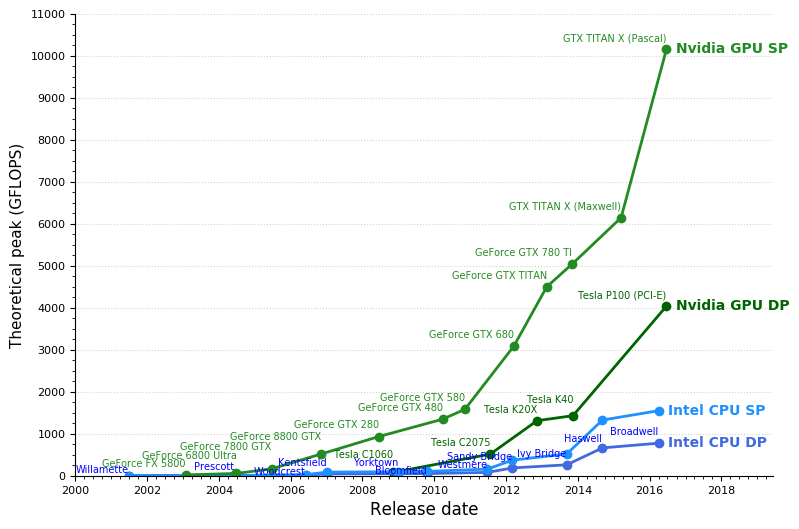
\includegraphics[width=\textwidth]{resources/graf.png}
\end{figure}